%%%% =================================================================
%%%% =================================================================
%%%% TEMPLATE FOR A SEMINAR PAPER 
%%%% AT THE INSTITUTE OF THEORETICAL COMPUTER SCIENCE 
%%%% AT THE UNIVERSITY OF ULM
%%%% 
%%%% AUTHOR
%%%% Florian Wörz <florian.woerz@uni-ulm.de>
%%%%
%%%% Based on earlier work by
%%%% Oliver Gableske, Dominikus Krüger, Simon Straub, Gunnar Völkel. 
%%%% 
%%%% VERSION
%%%% Last updated 2021/03/22.
%%%%  
%%%% =================================================================
%%%% =================================================================



%%%%%%%%%%%%%%%%%%%%%%%%%%%%%%%%%%%%%%%%%%%%%%%%%%%%%%%%%%%%%%%%%%%%%%
%%%% SETUP --- PLEASE INSERT YOUR INFORMATION!                    %%%%
%%%% Please sort the collaborators by last name!                  %%%%
%%%% If there is only one author, please replace the line         %%%%
%%%%     \newcommand{\SecondStudentName}{Second StudentB}         %%%%
%%%% with                                                         %%%%
%%%%     \newcommand{\SecondStudentName}{}                        %%%%
%%%% You can break the title of your report by using \\           %%%%
%%%%%%%%%%%%%%%%%%%%%%%%%%%%%%%%%%%%%%%%%%%%%%%%%%%%%%%%%%%%%%%%%%%%%%

\newcommand{\FirstStudentName}{First Student}
\newcommand{\FirstStudentMail}{first.student@uni-ulm.de}

% Replace with \newcommand{\SecondStudentName}{} if there is only one author
\newcommand{\SecondStudentName}{Second Student} 
\newcommand{\SecondStudentMail}{second.student@uni-ulm.de}

\newcommand{\TitleOfYourTopic}{Here you can insert the title of \\ your seminar paper}



%%%%%%%%%%%%%%%%%%%%%%%%%%%%%%%%%%%%%%%%%%%%%%%%%%%%%%%%%%%%%%%%%%%%%%
%%%% PREAMBLE STUFF --- DO NOT EDIT THIS PART!                    %%%%
%%%% To keep the template intact, this part should not be edited! %%%%
%%%%%%%%%%%%%%%%%%%%%%%%%%%%%%%%%%%%%%%%%%%%%%%%%%%%%%%%%%%%%%%%%%%%%%

% Specify the article class and paper format
\documentclass[a4paper]{article} 

% Use German identifiers, i.e., use "Zusammenfassung" instead of "Abstract" and "Literatur" instead of "References".
% Furthermore hyphenation rules will use heuristics of the German language.
\usepackage[ngerman]{babel} 
\usepackage[fixlanguage]{babelbib}

% Specify the encoding such that we can use German special characters (like Umlauts ä,ö,ü).
% Alternatively one can e.g. write ' f\"ur ' instead of ' für '.
\usepackage[utf8]{inputenc} 

% For the use of color in the document
\usepackage{color}

% Package for including graphics with the figure-environment
\usepackage{graphicx}

% Package for typesetting pseudo code
\usepackage[boxed]{algorithm2e}

% Tools for setting math formulas, use theorem environments, etc.
\usepackage{amsmath,amsthm,amssymb}

% Set Theorems, etc. in cursive
\theoremstyle{plain}
	\newtheorem{theorem}{Theorem}
	\newtheorem{satz}[theorem]{Satz}
	\newtheorem{lemma}[theorem]{Lemma}
	\newtheorem{proposition}[theorem]{Proposition}
	\newtheorem{corollary}[theorem]{Korollar}
% Set Definitions, etc. upright
\theoremstyle{definition}
	\newtheorem{definition}[theorem]{Definition}
	\newtheorem{claim}[theorem]{Behauptung}
	\newtheorem{remark}[theorem]{Bemerkung}
	\newtheorem{example}[theorem]{Beispiel}

% Package for using links in the document. We also specify the colors for the links
\usepackage{hyperref}
\hypersetup{bookmarks=true,
			bookmarksnumbered=true,
			pagebackref=true,
			colorlinks=true,
			linkcolor=red,
			citecolor=blue,
			filecolor=black,
			urlcolor=black}

% Package for page headers
\usepackage[automark]{scrpage2}
	\pagestyle{scrheadings}
	\ihead[]{%
		\ifdefempty{\SecondStudentName}{%
			\FirstStudentName
		}{%
	 		\FirstStudentName{} \& \SecondStudentName
 		}%
 	}
	\ohead[]{\today}
	\cfoot[]{\pagemark} 
	\setheadsepline[122mm]{0.3mm}

% Use for switching the design of the cover page in case of one/two authors	
\usepackage{etoolbox}	

% Set up the design of captions
\usepackage[font=footnotesize,
		    labelfont=bf,
            justification=justified,
            format=plain,
            margin=1.5cm]{caption}

% Allows strict placements of floats with the `H` option (\begin{figure}[H])
\usepackage{float}


	
%%%%%%%%%%%%%%%%%%%%%%%%%%%%%%%%%%%%%%%%%%%%%%%%%%%%%%%%%%%%%%%%%%%%%%
%%%% OWN COMMANDOS                                                %%%%
%%%% If you need to define own commands, please do so here.       %%%%
%%%% Examples are given below.                                    %%%%
%%%%%%%%%%%%%%%%%%%%%%%%%%%%%%%%%%%%%%%%%%%%%%%%%%%%%%%%%%%%%%%%%%%%%%	
	
% Complexity classes
\renewcommand{\P}{\mathsf{P}} % I suppose, we do not need the Polish character?
\newcommand{\NP}{\mathsf{NP}}

% Languages / Problems
\newcommand{\SAT}{\textnormal{SAT}}
\newcommand{\kSAT}{k{\text{-}}\SAT}	
	
% Mathematical Operators
\DeclareMathOperator{\arsinh}{arsinh} % So kann man "arsinh" als Matheoperator definieren. Die wird im "Mathemodus" dann aufrecht und nicht kursiv gesetzt.



%%%%%%%%%%%%%%%%%%%%%%%%%%%%%%%%%%%%%%%%%%%%%%%%%%%%%%%%%%%%%%%%%%%%%%
%%%% INSERT THE TITLE --- DO NOT EDIT!                            %%%%
%%%% We take care of the title page here.                         %%%%
%%%% To specify the title and the authors of your report, please  %%%%
%%%% use the commandos provided at the beginning of the document  %%%%
%%%%%%%%%%%%%%%%%%%%%%%%%%%%%%%%%%%%%%%%%%%%%%%%%%%%%%%%%%%%%%%%%%%%%%

\begin{document}
	
	\title{
		\begin{figure}[!ht]
			\centering
				
\includegraphics[width=0.5\textwidth]{logo_uulm_sw}
		\end{figure}
		\vspace{1cm}
		\Huge \TitleOfYourTopic 
	}
	
	
	\vspace{1cm}
	
	
	\ifdefempty{\SecondStudentName}{%
		\author{%
		\Large \href{mailto:\FirstStudentMail}{\FirstStudentName}
		\vspace{1cm}
		}%
	}{%
		\author{%
			\Large \href{mailto:\FirstStudentMail}{\FirstStudentName} \and \Large \href{mailto:\SecondStudentMail}{\SecondStudentName}
			\vspace{1cm}
		}%
	}%
	
	
	\date{
		\large Seminar: Einführung in die Algorithmik \\ \textit{Algorithmen in der Aussagenlogik und Beweiskomplexität} \\ 
		\vspace{0.8cm}
		\large Betreuer: Jacobo Torán und Florian Wörz \\
		\vspace{1cm}
		\today
	}

	\maketitle



%%%%%%%%%%%%%%%%%%%%%%%%%%%%%%%%%%%%%%%%%%%%%%%%%%%%%%%%%%%%%%%%%%%%%%
%%%% INSERT THE ABSTRACT --- PLEASE DO EDIT!                      %%%%
%%%% Please insert the abstract (Zusammenfassung) of your report  %%%% 
%%%% here. Keep it short! The Abstract has to fit on the first    %%%%
%%%% page. You might want to replace                              %%%%
%%%%     \vspace{2em}                                             %%%%
%%%% by a smaller number in the brackets or by                    %%%%
%%%%     \vfill                                                   %%%%
%%%%%%%%%%%%%%%%%%%%%%%%%%%%%%%%%%%%%%%%%%%%%%%%%%%%%%%%%%%%%%%%%%%%%%

\vspace{2cm}

\begin{abstract}
	Lorem ipsum dolor sit amet, consetetur sadipscing elitr, sed diam nonumy eirmod tempor invidunt ut labore et dolore magna aliquyam erat, sed diam voluptua. At vero eos et accusam et justo duo dolores et ea rebum. Stet clita kasd gubergren, no sea takimata sanctus est Lorem ipsum dolor sit amet. Lorem ipsum dolor sit amet, consetetur sadipscing elitr, sed diam nonumy eirmod tempor invidunt ut labore et dolore magna aliquyam erat, sed diam voluptua. At vero eos et accusam et justo duo dolores et ea rebum. Stet clita kasd gubergren, no sea takimata sanctus est Lorem ipsum dolor sit amet.
\end{abstract}



%%%%%%%%%%%%%%%%%%%%%%%%%%%%%%%%%%%%%%%%%%%%%%%%%%%%%%%%%%%%%%%%%%%%%%
%%%% INSERT THE TABLE OF CONTENTS --- DO NOT EDIT!                %%%%
%%%% LaTeX will automatically insert it for you if you use the    %%%% 
%%%% correct sectioning commands like                             %%%% 
%%%%     \section{Section}                                        %%%% 
%%%%     \subsection{Subsection}                                  %%%% 
%%%%     \subsubsection{Subsubsection}                            %%%% 
%%%%     \paragraph{Paragraph}                                    %%%% 
%%%% You probably shouldn't use \subparagraph{...} for such a     %%%% 
%%%% short document.                                              %%%% 
%%%%%%%%%%%%%%%%%%%%%%%%%%%%%%%%%%%%%%%%%%%%%%%%%%%%%%%%%%%%%%%%%%%%%%

\newpage

% Change the settings of linkcoloring locally: Do not print links red in TOC
{
	\hypersetup{linkcolor=black}
	\tableofcontents
}

\newpage



%%%%%%%%%%%%%%%%%%%%%%%%%%%%%%%%%%%%%%%%%%%%%%%%%%%%%%%%%%%%%%%%%%%%%%
%%%% INSERT THE CONTENT OF YOU REPORT HERE                        %%%%
%%%% Now we have arrived at the main body of the document.        %%%%
%%%% Replace the example below with your text.                    %%%%
%%%% Please be careful not to erase the commands for the          %%%%
%%%% bibliography at the end of the document!                     %%%%
%%%%%%%%%%%%%%%%%%%%%%%%%%%%%%%%%%%%%%%%%%%%%%%%%%%%%%%%%%%%%%%%%%%%%%


%=====================================================================
\section{Einleitung}
%=====================================================================

Eure Arbeit braucht eine \emph{Einleitung}, welche dem Leser einen \"Uberblick \"uber das Thema gibt. Es bietet sich an hier auch \glqq related work\grqq{} abzuhandeln -- also wichtige Vorarbeiten, die man sich eventuell anschauen muss. Im Quelltext könnt ihr sehen, wie kursiv hervorgehoben wird (wir unterstreichen nichts!), sowie deutsche Anführungszeichen und Gedankenstriche gesetzt werden (immer als Halbgeviertstriche im Deutschen!).


%=====================================================================
\section{Hauptteil}
%=====================================================================

Danach geht es an den Hauptteil. F\"ur gew\"ohnlich werden im Hauptteil zun\"achst die Formalismen abgehandelt. So m\"usst ihr hier z.\,B. relevante Definitionen liefern und k\"onnt auch gleich das eine oder andere Lemma angeben (und i.\,d.\,R. beweisen). Beachte: Abkürzungen, wie z.\,B. werden mit halben Leerzeichen gesetzt! Evtl. könnt ihr euch ja hierfür eine eigene Abkürzung definieren. Danach verwendet ihr die eingef\"uhrten Begrifflichkeiten, um das Problem zu beschreiben und einen L\"osungsansatz vorzustellen (oftmals in Form von evtl.\ mehreren Algorithmen).

%---------------------------------------------------------------------
\subsection{Definitionen}
%---------------------------------------------------------------------

Eine Definition wird normalerweise besonders gekennzeichnet (\"ubertreibt dies nicht, Trivialit\"aten wie unten will man normalerweise nicht in einer wissenschaftlichen Arbeit sehen).

\begin{definition}[Die nat\"urlichen Zahlen und Summen]
	Im folgenden bezeichnen wir die \emph{nat\"urlichen Zahlen} mit dem Symbol $\mathbb{N}$. Die Zahl~$0$ ist nicht in $\mathbb{N}$ enthalten. Die \emph{Summe zweier natürlicher Zahlen} $a,b \in \mathbb{N}$ notieren wir mit $a+b$.
\end{definition}

Hier beginnt ein neuer Absatz. Man sieht dies am Einzug. Definitionen k\"onnen unter Umst\"anden sehr lang werden. Wichtig ist, dass im Rahmen einer Definition alle verwendeten Symbole eingef\"uhrt werden. Normalerweise definiert man Begriffe, um diese im Text oder in Lemmata und Theoremen verwenden zu k\"onnen. Wichtig ist ebenfalls eine Definition nicht mit einem Satz zu vermischen.

%---------------------------------------------------------------------
\subsection{Lemmata, Theoreme und Korollare mit und ohne Beweis}
%---------------------------------------------------------------------

Der Unterschied zwischen Lemmata, Theoremen, und Korollaren ist wie folgt.

\begin{lemma}
	Im Folgenden bezeichnen wir einen Hilfssatz, der eine vergleichsweise einfache Aussage oder Einsicht feststellt, als ein \emph{Lemma}. Oftmals sind Beweise zu Lemmata nur wenige Zeilen lang. 
\end{lemma}

Wollen wir ein Lemma (oder andere Matheumgebungen wie Definition, Theorem, o.\,Ä.) besonders benennen, so ist dies auch möglich.

\begin{lemma}[Lemma von Fatou]
	Das Lemma von Fatou ist eine Aussage aus der Maßtheorie.
\end{lemma}

\begin{theorem}
	\label{def:irgendeinedefinition}
	Weiterhin bezeichnen wir zentrale Aussagen, die zumei\ss t lange und recht komplexe Beweise ben\"otigen, als ein \emph{Theorem} (oder einen \emph{Satz}). Vergleichsweise h\"aufig werden zum Beweisen von Theoremen diverse Lemmata angewendet.
\end{theorem}

\begin{satz}
	Dies ist ein Satz. Ein Satz ist nicht ganz so wichtig wie ein Theorem. Theorem sind die zentralen Aussagen der Arbeit. Es sollte nur wenige Theoreme geben.
\end{satz}

\begin{remark}
	Das ist eine Bemerkung. Sie ist aufrecht gesetzt.
\end{remark}

\begin{corollary}
	Zu guter Letzt bezeichnen wir einfache Aussagen, die sich direkt aus Theoremen oder Lemmata ergeben als \emph{Korollare}. Korollare folgen oft als Spezialf\"alle von allgemeiner formulierten S\"atzen. 
\end{corollary}

Eine einfacher Hilfssatz kann wie folgt aussehen.

\begin{lemma}
	Seien $a, b \in \mathbb{N}$ und sei $c := a+b$, so ist $c \geq a$ und $c \geq b$.
\end{lemma}

\begin{proof}
	Wir führen einen Beweis durch Widerspruch unter der Annahme $c < a$ (der Fall $c<b$ folgt analog). Dann wäre
		\begin{align}
		c < a \Longleftrightarrow  a + b - a < 0 \Longleftrightarrow b < 0.
		\end{align}
	Widerspruch zur Voraussetzung mit $b \in \mathbb{N}$ wegen Definition~\ref{def:irgendeinedefinition}. Man beachte die Referenz auf die Definition und das \glqq Beweisendezeichen\grqq{} auf der rechten Seite (wird automatisch generiert). Die Referenznummer binden wir mit einer Tilde an das Wort \glqq Definition\grqq{}, um einen Zeilenumbruch an dieser Stelle zu verhindern! Die Referenz ist klickbar und rot eingefärbt.
\end{proof}

Theoreme und Korollare k\"onnen in analoger Weise gesetzt werden. M\"ochte man einen Beweis weglassen (weil zu trivial oder kein Platz) so l\"asst man einfach die Beweisumgebung weg.\\

\textbf{Ganz wichtig:} Text in Definitionen, Beispielen, etc. wird aufrecht gesetzt (mit dem zu definierenden Wort kursiv); Text in Sätzen, Lemmata, Theoremen, etc. wird kursiv gesetzt.

%---------------------------------------------------------------------
\subsection{Formeln}
%---------------------------------------------------------------------

Das Textsatzsystem \LaTeX{} wurde entwickelt, um die wissenschaftliche Textverarbeitung zu erleichtern. Dazu geh\"ort, dass man Formeln in angemessener Art und Weise setzen kann. Dies kann wie folgt geschehen (zweizeilig):
	\begin{align}
	\mathcal{H}_{T,n}
	&= \frac{1}{n}\ln \left[\sum_{\nu\in\mathbb{S}^n} e^{-E_{SK}(\nu)/T}\right]\\
	&= \frac{1}{n}\ln \left[\sum_{\nu\in\mathbb{S}^n}\hspace{-0.1cm}\exp\left( \frac{1}{T}\sum_{\{i,j\}\in C}\hspace{-0.2cm}J_{i,j}\nu_i\nu_j + \frac{M}{T} \sum_{i=1}^n\nu_i\right) \right].
	\end{align}
Oder aber:
	\begin{align}
	\pi = 4\cdot\arctan(1) \approx 3.14159265359\label{eqn:pi}.
	\end{align}

	
Jetzt eine unnummerierte Gleichung (bitte nur Gleichungen nummerieren, die auch referenziert werden):
	\[
	\text{Text im Gleichungsmodus: } a_1 \cdot \ldots \cdot a_n = \prod_{i=1}^n a_i.
	\]
Und hier unser eigens definierter Operator (siehe Quellcode):
	\[
	\arsinh x = \log (x + \sqrt{x^2 + 1}).
	\]
Wir benutzen Klammern nur, wenn es nötig ist.
	
Man beachte: Es ist auch m\"oglich logische Operationen oder Quantoren zu verwenden.
	\begin{align}
	F \in \SAT 
	:\!\iff 
	\exists \alpha \colon \: \forall C \in F \colon \: \exists \ell \in C \colon \: \alpha(\ell) = 1.
	\end{align}
Hier etwas Logik:
	\[
	F = (v_1 \lor v_2 \lor v_3) \land (\neg v_1 \lor \neg v_2 \lor \neg v_3).
	\]
Wichtig: Für ein \glqq ell\grqq{} schreiben wir im Mathemodus niemals $l$ (Verwechslungsgefahr!), sondern $\ell$.
Manchmal ist es hilfreich, wenn man eine Formel im Text referenziert. Beispielsweise zeigt Gleichung~\eqref{eqn:pi} wie man mit jeder halbwegs modernen Programmiersprache die Kreiszahl $\pi$ n\"aherungsweise bestimmen kann. Für die Referenz einer Gleichung benutzt man \verb|\eqref{label}| -- damit werden direkt die runden Klammern gesetzt.

Mathematische Ausdrücke in einem Fließtext 
können durch zwei \$ Zeichen eingebunden werden.
So wird die Formel $f(n)=\sum_{i=1}^n i$ durch 
den Ausdruck \verb|$f(n)=\sum_{i=1}^n i$| erzeugt.
Soll die Formel vom Fließtext abgehoben werden, wie
zum Beispiel 
	\begin{equation*}
	f(n)=\sum_{i=1}^n i,
	\end{equation*} 
kann das durch \verb|\begin{equation*} ... \end{equation*}| gewonnen
werden.

Analog erfolgt die Verwendung von Lemmata, Definitionen, usw.:
	\begin{verbatim}
	\begin{lemma}[optional mit Titel]
	Hier steht das Lemma.
	\end{lemma}
	\end{verbatim}

Sicherlich sind viele weitere Dinge über \LaTeX~zu 
erwähnen. Das Internet wird aber die meisten Fragen
beantworten können. 
Wie genau z.\,B. die Befehle f\"ur bestimmte Symbole sind, k\"onnt ihr im Internet nachsehen\footnote{Lohnenswert ist auch nach \glqq Detexify \LaTeX{} handwritten symbol recognition\grqq{} zu googeln. Das ist übrigens eine Fußnote!}. Siehe beispielsweise \url{https://de.wikipedia.org/wiki/Hilfe:TeX}.

%---------------------------------------------------------------------
\subsection{Referenzen, Quellen, Literatur}
%---------------------------------------------------------------------

In einem wissenschaftlichen Artikel m\"ussen alle Quellen, mit denen der Autor gearbeitet hat, klar angegeben werden. Weiterhin m\"ussen alle wesentlichen Aussagen (wie Lemmata, Theoreme, oder Abbildungen) mit einer Quelle belegt werden (falls der Autor diese Aussage nicht selbst erarbeitet hat). Das simple Kopieren von Bildern ist in der Regel nicht zulässig. Das \glqq Belegen mit einer Quelle\grqq{} erfolt durch ein Zitat. Es kann bisweilen vorkommen, dass man mehr als eine Quelle angeben muss.

\begin{theorem}[Cook-Levin Theorem, \cite{Cook71TheComplexityOf, Levin73UniversalSearchProblems}] 
	Die Sprachen $\SAT$ und $\kSAT$ (mit $k\geq 3$) sind $\NP$-vollst\"andig.
\end{theorem}

Soll eine Aussage im Flie\ss text belegt werden so gen\"ugt es das Zitat an das Ende des Satzes oder des Paragraphen zu stellen~\cite{Cook71TheComplexityOf}. Quellen referenziert man mit \verb|\cite{...}|. Das Literaturverzeichnis ist hier in der externen Datei \verb|references.bib| hinterlegt. Der Inhalt der Datei:
	\begin{verbatim}
	@inproceedings{Cook71TheComplexityOf,
	author    = {Stephen A. Cook},
	title     = {The Complexity of Theorem-Proving Procedures},
	booktitle = {Proceedings of the 3rd Annual {ACM} Symposium 
	             on Theory of Computing ({STOC}~'71)},
	pages     = {151\nobreakdash--158},
	year      = {1971},
	url       = {https://doi.org/10.1145/800157.805047},
	doi       = {10.1145/800157.805047},
	}
	
	@article{Levin73UniversalSearchProblems,
	author    = {Levin, Leonid A.},
	title     = {Universal Search Problems},
	journal   = {Problems of Information Transmission},
	number    = {3},
	volume    = {9},
	pages     = {115\nobreakdash--116},
	year      = {1973},
	}
	
	@book{ST12SAT,
	author    = {Uwe Sch{\"{o}}ning and
	Jacobo Tor{\'{a}}n},
	title     = {Das Erf{\"{u}}llbarkeitsproblem {SAT} -- 
	             Algorithmen und Analysen},
	series    = {Mathematik f{\"{u}}r Anwendungen},
	volume    = {1},
	publisher = {Lehmann},
	year      = {2012},
	}
	\end{verbatim}

Das Literaturverzeichnis ist dann am Ende der Arbeit eingebunden. Hier ein Beispielzitat für ein Buch:~\cite{ST12SAT}.
Um Literaturangaben zu bekommen empfiehlt sich \url{https://dblp.uni-trier.de/}. Die Einträge kann man als BibTeX exportieren. Der Originaleintrag für~\cite{Cook71TheComplexityOf} sieht zum Beispiel wie folgt aus:
	\begin{verbatim}
	@inproceedings{DBLP:conf/stoc/Cook71,
	author    = {Stephen A. Cook},
	title     = {The Complexity of Theorem-Proving Procedures},
	booktitle = {Proceedings of the 3rd Annual {ACM} Symposium
	             on Theory of Computing,
	             May 3-5, 1971, Shaker Heights, Ohio, {USA}},
	pages     = {151--158},
	year      = {1971},
	crossref  = {DBLP:conf/stoc/STOC3},
	url       = {https://doi.org/10.1145/800157.805047},
	doi       = {10.1145/800157.805047},
	timestamp = {Mon, 26 Nov 2018 15:05:57 +0100},
	biburl    = {https://dblp.org/rec/conf/stoc/Cook71.bib},
	bibsource = {dblp computer science bibliography, https://dblp.org}
	}
	\end{verbatim}
Wie man sieht sind oft \glqq unnötige\grqq{} Informationen wie \verb|timestamp|, \verb|biburl|, \verb|bibsource| enthalten. Man sollte auf jeden Fall den \verb|booktitle| bei Proceedings (Konferenzbände) in ein einheitliches Format bringen. Wir verwenden das folgende, bewährte Format (für eine Konferenz im Jahre 1999):
	\begin{verbatim}
	Proceedings of the nth Conference on Some Topic 
	({GROSSBUCHSTABENABKUERZUNG}~'99)
	\end{verbatim}
Insbesondere lassen wir den Austragungsort und das Austragungsdatum der Konferenz weg.

%---------------------------------------------------------------------
\subsection{\"Ubersetzung der TeX-Datei in eine PDF-Datei}
\label{uebersetzung}
%---------------------------------------------------------------------

Ein pdf-Dokument wird z.\,B. mit einer Kommandozeile durch den Befehl 
	\begin{verbatim}
	pdflatex ausarbeitung.tex
	\end{verbatim}
generiert. Damit alle Referenzen korrekt aufgelöst werden (wie bspw. die Referenz auf die Definition oben oder die Referenz auf eine Quelle), ist in der Regel eine zweifache \"Ubersetzung notwendig. \TeX studio oder ähnliche Programme machen euch das Leben leichter!

%---------------------------------------------------------------------
\subsection{Weitere Formatbefehle}
%---------------------------------------------------------------------

Eine Aufzählung lässt sich realisieren z.\,B. mit:
	\begin{enumerate}
		\item Erstens
		\item Zweitens
	\end{enumerate}
Bulletpoints mit
	\begin{itemize}
		\item Erstens 
		\item Zweitens
	\end{itemize}
Eine Description mit
	\begin{description}
		\item[Stichwort] Text.
		\item[Anderes Stichwort] Wichtiger Text.
	\end{description} 


%=====================================================================
\section{Abbildungen}
%=====================================================================

Man kann in \LaTeX{} ganz bequem Abbildungen einsetzen.

\begin{figure}[h!]
	\centering
	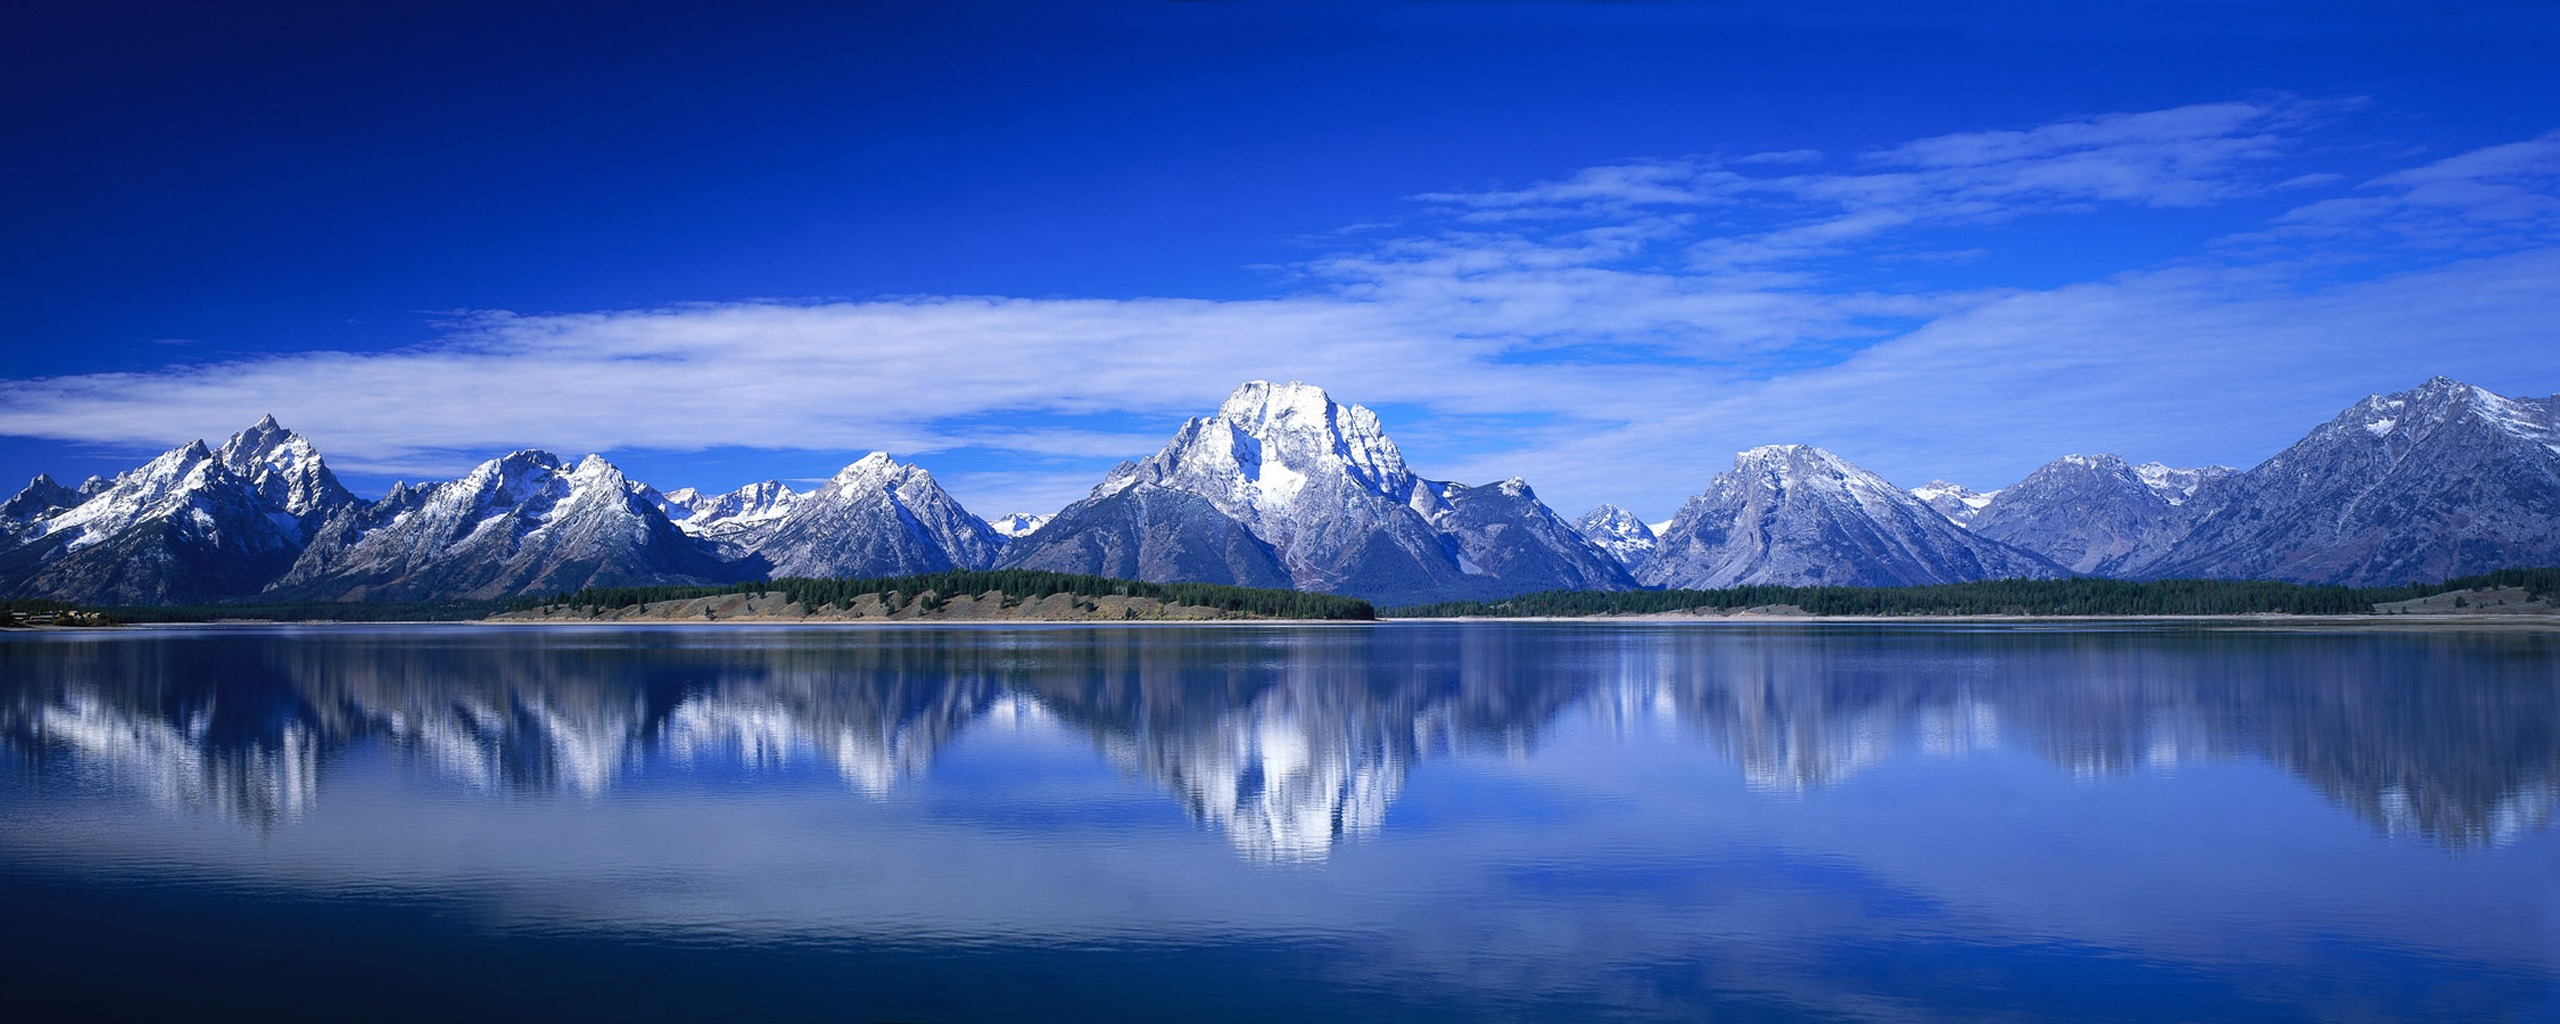
\includegraphics[width=0.75\textwidth]{bild.jpg}
	\caption{Testunterschrift. Lots-of-text wird von \LaTeX{} automatisch umgebrochen und mit ausreichen Abstand zum Folgetext versehen. \label{bild:label}}
\end{figure}

Solche Bilder wie in Abbildung~\ref{bild:label} gezeigt m\"ussen nicht im \texttt{JPG}-Format vorliegen. Man kann auch \texttt{PNG}, \texttt{PDF}, etc. verwenden. Weitere Informationen findet man z.\,B. auf der Seite \url{https://en.wikibooks.org/wiki/LaTeX/Floats,_Figures_and_Captions}. Solltet ihr Abbildungen aus anderen Arbeiten oder dem Internet \"ubernehmen wollen, so \emph{m\"usst} ihr diese selber nachzeichnen. Einfach copy-and-paste ist aus Urheberrechtsgr\"unden nicht erlaubt. Referenzieren m\"usst ihr die Quelle in jedem Fall.


%=====================================================================
\section{Pseudocode}
%=====================================================================

Weiterhin kann man ganz bequem Pseudocode einsetzen. Siehe hierzu Algorithmus~\ref{algo:StudentenArtikelLeseAlgo}. Eine vollständige Einführung findet sich in der Dokumentation \url{https://ctan.org/pkg/algorithm2e} von \verb|Algorithm2e|.

\begin{figure}
	\begin{algorithm}[H]
		%\dontprintsemicolon
		\KwData{Artikel}
		\KwResult{Wie viele Abschnitte verstanden wurden}
		Initialisierung:\\
		$u := 0$\\
		der erste Abschnitt wird der momentane Abschnitt\\
		\While{nicht am Dokumentende angelangt}{
			lese den momentanen Abschnitt\\
			\eIf{Abschnitt verstanden}{
				gehe zum n\"achsten Abschnitt\\
				der n\"achste Abschnitt wird der momentane Abschnitt\\
				erh\"ohe den Verst\"andnisz\"ahler $u := u + 1$
			}{
				gehe zur\"uck zum Anfang des Abschnitts
			}
		}
		\Return $u$\\[0.2cm]
		\caption{Der Studenten-Artikel-Lese-Algorithmus.}
		\label{algo:StudentenArtikelLeseAlgo}
	\end{algorithm}
\end{figure}

Verwendet im Pseudocode bitte keine Terminationssymbole wie \glqq;\grqq{} oder \"Ahnliches. Der Mensch ist kein Compiler! Zudem soll Pseudocode die wesentliche Idee hinter einem Algorithmus verdeutlichen. Setzt bitte keine Programme die man tats\"achlich kompilieren kann!


%=====================================================================
\section{Tabellen}
%=====================================================================

Tabellen kann man wie folgt setzen.
\begin{table}[h!]
	\centering
	\begin{tabular}{|c|cc|cccc|}
		\hline
		\textbf{Head1}& \textbf{Head2}& \textbf{Head3}& \textbf{Head4}& \textbf{Head5} &\textbf{Head6}  & \textbf{Head7}\\
		\hline 
		1 & stuff & aoeuc & eoiaeo & aoeuaoeua & $1234567890$ & Text. \\
		\hline
		2 & stuff & 3\&4c & eoiaeo & 3\&4c & eoiaeo & 3\&4c \\ 
		\hline 
	\end{tabular}
	\caption{Stuff.}
\end{table}

Auch hier gilt: Solltet ihr Tabellen aus anderen Arbeiten \"ubernehmen wollen so \emph{m\"usst} ihr diese selber nachbauen und dann \emph{unbedingt referenzieren}.

Sind wir ehrlich, müssen wir uns eingestehen: Die obige Tabelle ist hässlich! Daher verwendet ihr am besten \verb|booktabs|.\footnote{Siehe die Präsentation \url{https://www.inf.ethz.ch/personal/markusp/teaching/guides/guide-tables.pdf}.}


%=====================================================================
\section{Ausblick}
%=====================================================================

Am Schluss der Ausarbeitung kommt gegebenenfalls ein Ausblick. 
Hier kann zum Beispiel auch auf Schw\"achen und St\"arken des Ansatzes eingegangen werden. 
Offene Fragen und m\"ogliche Weiterentwicklungen sind angebracht.



%%%%%%%%%%%%%%%%%%%%%%%%%%%%%%%%%%%%%%%%%%%%%%%%%%%%%%%%%%%%%%%%%%%%%%
%%%% INSERT BIBLIOGRAPHY --- DO NOT EDIT (ONLY TO SWITCH LANGUAGE)! %%
%%%% To cite something, modify the example file `references.bib`.   %%
%%%%%%%%%%%%%%%%%%%%%%%%%%%%%%%%%%%%%%%%%%%%%%%%%%%%%%%%%%%%%%%%%%%%%%

\newpage 

\bibliography{references}
%\bibliographystyle{alpha} % If one uses English, uncomment this line and comment the next one
\bibliographystyle{babunsrt}
\addcontentsline{toc}{section}{Literatur}


\end{document}